\chapter{Oracle}

\section{Introduzione}

Oracle e' una societa' che mette a disposizione numerosi prodotti, per la parte di confronto relazionale e' stato usato oracle SQL developer, un software opensource che 
mette a disposizione un software per poter lavorare con SQL su database di Oracle attraverso il JDK (java development kit).

\section{Raccolta dati}

\section{Organizzazione dei dati}

Utilizzando un sistema relazionale ci si e' dovuti limitare alla crezione di due collezioni distinte A (Post) e B(Commenti) sulle quali eseguire le query di selezione per poter
ottenere una stima dei costi su un modello relazionale che non utlizasse embedding e referencing.

Sono stati creati file .csv dei dati facilmente importabili in un database Oracle creato su un computer fisso, sui quali sono state effettuate alcune operazioni come la creazione di 
indici per specifici attributi e la limitazione della memoria cache del database locale. 

\begin{minted}[]{sql}
        -- Primary key per A

        alter table "SYS"."A" add constraint PK primary key("AK") 

        -- Primary key per B

        alter table "SYS"."B" add constraint PKB primary key("BK") 

        -- Aggiungere il constraint per FAK

        ALTER TABLE B
          ADD CONSTRAINT FK_A_constr FOREIGN KEY (FAK)     
              REFERENCES A(AK)
              ON DELETE CASCADE;

        -- Indici

        CREATE BITMAP INDEX A_A4_BITMAP ON A (A4 ASC);
        CREATE BITMAP INDEX A_A5_BITMAP ON A (A5 ASC);
        CREATE BITMAP INDEX A_A6_BITMAP ON A (A6 ASC);
        CREATE BITMAP INDEX B_B4_BITMAP ON B (B4 ASC);
        CREATE BITMAP INDEX B_B5_BITMAP ON B (B5 ASC);
        CREATE BITMAP INDEX B_B6_BITMAP ON B (B6 ASC);
        CREATE BITMAP INDEX B_FK_BITMAP ON B (FAK ASC);

        -- Ridurre la cache del client di sistema

        ALTER SYSTEM SET CLIENT_RESULT_CACHE_SIZE = 128M SCOPE=SPFILE;
 
\end{minted}


\section{Inserimento (CRUD: Creation)}


Oracle è un database relazionale, sul quale risulta semplice inserire una tupla all'interno di una tabella attraverso PL/SQL ma nel caso di una quantità
cospiqua di dati non è piu possibile utilizzare quel metodo che funziona nei piccoli numeri. Il software non riesce a completare quei task cosi ci si è 
appoggiati alla funzionalità di importazione da file, in particolare si è adattato il dataset ad essere un file di tipo .csv che è stato facilmente 
inserito all'interno dell'istanza del database.

\begin{center}
    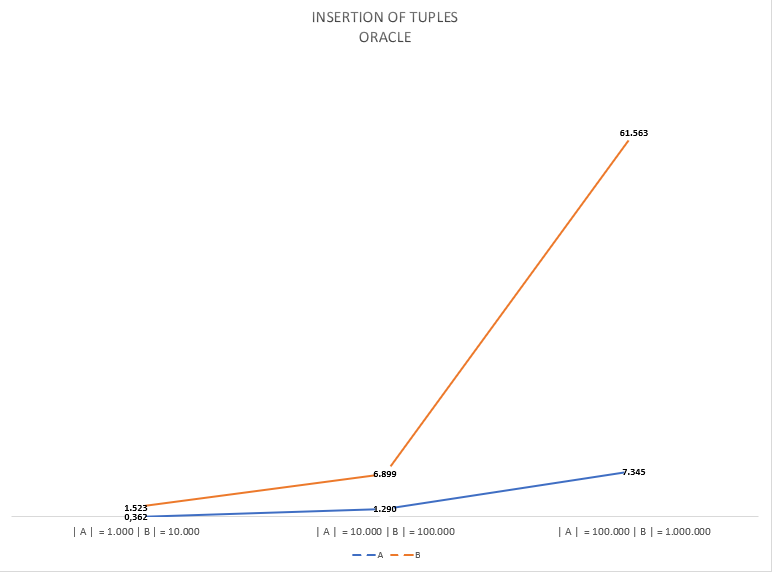
\includegraphics[scale=0.8]{InsertionOracle.png}
\end{center}

//TODO server section


\section{Selezione (CRUD: Read)}

Per poter eseguire le query di selezione e' stato utilizzato uno script in python che utilizza il modulo \verb|cx_Oracle| per poter creare una connessione 
al database locale ed effettuare un numero arbitrario di query, ogni query effettuata riporta un piano di esecuzione visionabile nell'apposito file 
.sql. Dopo che la connessione viene confermata, si procede a creare 
un cursore con il quale si andranno ad eseguire query articolate come segue:

\begin{minted}[]{sql}
        EXPLAIN PLAN FOR SELECT * FROM A WHERE A6 = 612;
        SELECT PLAN_TABLE_OUTPUT FROM TABLE(DBMS_XPLAN.DISPLAY());
\end{minted}

Che provvedono ad esegure una query e scrivere una riga all'interno del \verb|PLAN_TABLE_OUTPUT| che poi verra letta e salvata 
in un file, per poter avere una copia del piano di esecuzione di ciascuna query.

\begin{table}[!ht]
    \centering
    \begin{tabular}{|l|l|l|}
    \hline
        ~ & A & B \\ \hline
        A0 & 15 & ~ \\ \hline
        A1 & 47 & ~ \\ \hline
        A2 & 17 & ~ \\ \hline
        A3 & 6 & ~ \\ \hline
        A4 & 4 & ~ \\ \hline
        A5 & 1 & ~ \\ \hline
        A6 & 1 & ~ \\ \hline
        B0 & ~ & 7 \\ \hline
        B1 & ~ & 295 \\ \hline
        B2 & ~ & 10 \\ \hline
        B3 & ~ & 5 \\ \hline
        B4 & ~ & 3 \\ \hline
        B5 & ~ & 5 \\ \hline
        B6 & ~ & 1 \\ \hline
        A0j & 5 & ~ \\ \hline
        A1j & 15 & ~ \\ \hline
        A2j & 3 & ~ \\ \hline
        A3j & 4 & ~ \\ \hline
        A4j & 3 & ~ \\ \hline
        A5j & 2 & ~ \\ \hline
        A6j & 3 & ~ \\ \hline
        B0j & ~ & 4 \\ \hline
        B1j & ~ & 524 \\ \hline
        B2j & ~ & 10 \\ \hline
        B3j & ~ & 937 \\ \hline
        B4j & ~ & 2 \\ \hline
        B5j & ~ & 5 \\ \hline
        B6j & ~ & 797 \\ \hline
    \end{tabular}
\end{table}


\section{Aggiornamento (CRUD: Update)}

Le query di aggiornamento dei dati hanno prodotto i seguenti risultati 